\documentclass[../main.tex]{subfiles}
\graphicspath{{\subfix{../img/}}}

\begin{document}

\subsection{Effects of T-Type Channel KD on Minimal Membrane Potential During Bursting}

\noindent An unpublished study of David Owald, Anatoli Ender, and colleagues reported increase in the minimal recorded membrane potential following knockdown of the T-type $\text{Ca}2+$ channels. This finding may seem counterintuitive, given that calcium current is depolarizing. Thus, reducing such a current would typically be expected to lower, not raise, the membrane potential. The observation suggests presence of an additional, potentially calcium-dependent, mechanism.

One possible class of mechanisms involves intracellular processes that depend on, or are triggered by calcium.
It has been demonstrated, that calcium can activate various signaling cascades in neurons, trigger transcriptional responses in neurons, and affect synaptic scaling \parencite{hagenstonFunctionalConsequencesCalciumDependent2020}. Therefore, a reduction in calcium infux due to T-type channel knockdown could, in principle, influence synaptic strength between R5 neurons,
or modulate their intrinsic properties (e.g. expression of other ion channels), thereby affecting the minimal membrane potential during bursting.

However, another potential mechanism that does not rely on calcium-dependent changes in intrinsic properties of neurons, is the involvement of calcium activated potassium channels. Since potassium currents are hyperpolarizing, their activation could contribute to the minimal membrane potential.  
A reduction in calcium influx could potentially lead to reduced activation of these potassium channels, resulting in less hyperpolarization, and, consequently, an increase in the minimal membrane potential. This thesis primarily focuses on this latter mechanism.

Considering the potential modulation of calcium-dependent synaptic strength, and the contribution of the T-type channels in activating calcium-activated potassium channels, across all implemented models, all parameters were held fixed (see the corresponding values in Appendix \ref{appendix:functions_and_parameters}), and only the input current and the maximal conductance of the T-type channels were varied. Note, that as discussed in Section \ref{sec:sleep_and_r5_network},
knockdown of the T-type channel could have been incomplete, hence the maximal conductance of these channels was systematically reduced, rather than set to $0$.

\afterpage{%

    \begin{figure}[!t]
        \centering
        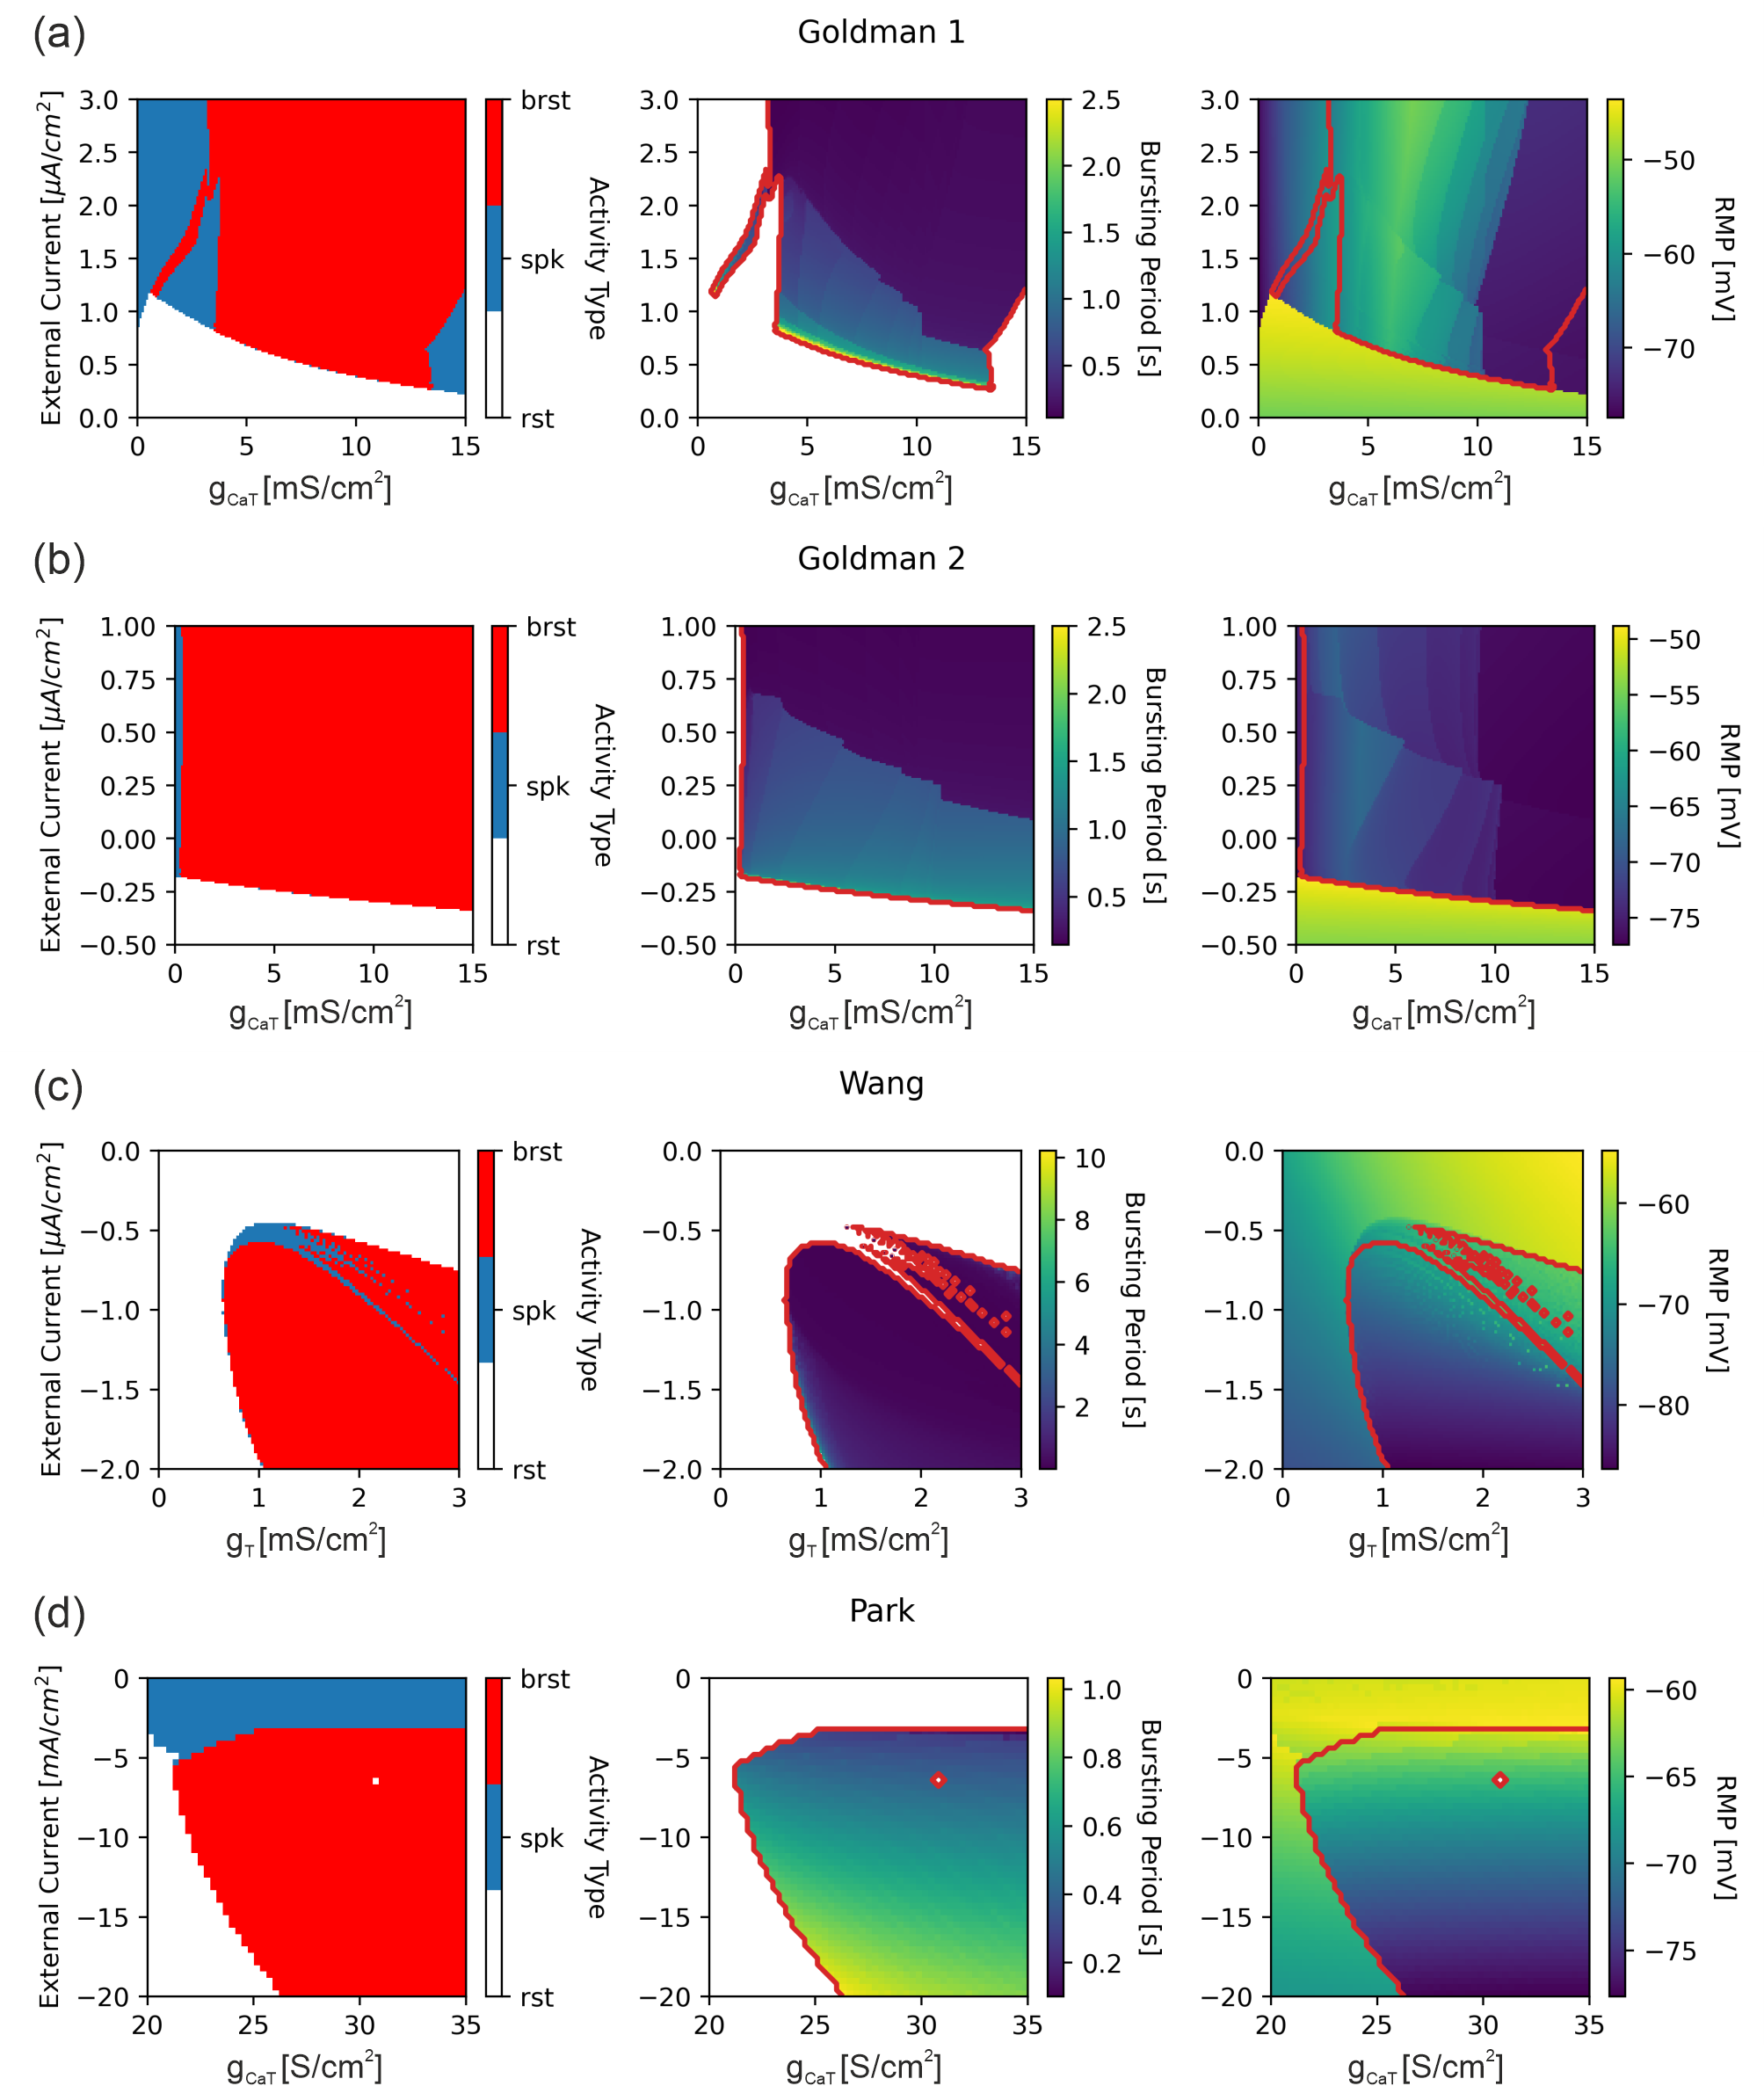
\includegraphics[width=0.9\linewidth]{../img/rmp/rmp_phase.png}
        \caption[Effect of T-type channel conductance and input current on minimal membrane potential]{\textbf{Effect of T-type channel conductance and input current on minimal membrane potential.} Results for the four implemented models. $x$-axis indicates the maximal conductance of T-type calcium channels, and the $y$-axis shows external input to the neuron. Labels and units match those described in Appendix \ref{appendix:functions_and_parameters}. Left: regions in the I$_\text{ext}$-$g$ parameter plane where models exhibit bursting (red), spiking (blue), or resting (white) activity. Middle: dependence of the bursting period on external input and mT-type channel conductance. Right: dependence of the minimal membrane potential on external input and T-type channel conductance. Regions in which the model exhibited bursting are outlined in red. \textcolor{red}{Period of Wang - change clims; RMP - min. V}}
        \label{fig:rmp_models_phase}
    \end{figure}

}

Figure \ref{fig:rmp_models_phase} shows the results for the four implemented models.
Note, that the labels on the $x$ axes, as well as the units have been selected to remain consistent with those used in the corresponding papers (see Appendix \ref{appendix:functions_and_parameters}), and both $g_{CaT}$ and $g_T$ refer to the maximal conductance of T-type calcium channels.

Interestingly, a reduction in the maximal conductance of the T-type channels was sufficient to increase the minimal membrane potential only in two of the models - Goldman 1 and Goldman 2. These models are characterized by a relatively high maximal conductance of calcium-activated potassium channels compared to that of the calcium channels (see Figure \ref{fig:model_conductances}).
In contrast, for the other two models, an increase in external current was necessary to elevate the minimal membrane potential.

Given that this thesis focuses on the role of calcium-activated potassium channels in modulating the minimal membrane potential, in the following, the analysis will focus on the two models in which a reduction in the maximal conductance of T-type channels resulted in increased minimal membrane potential.

\afterpage{%
\begin{figure}[!t]
    \centering
    \textbf{Goldman 1 Model} \\[1ex]  % Title at top center
    % First row
    \begin{subfigure}[t]{0.48\textwidth}
        \centering
        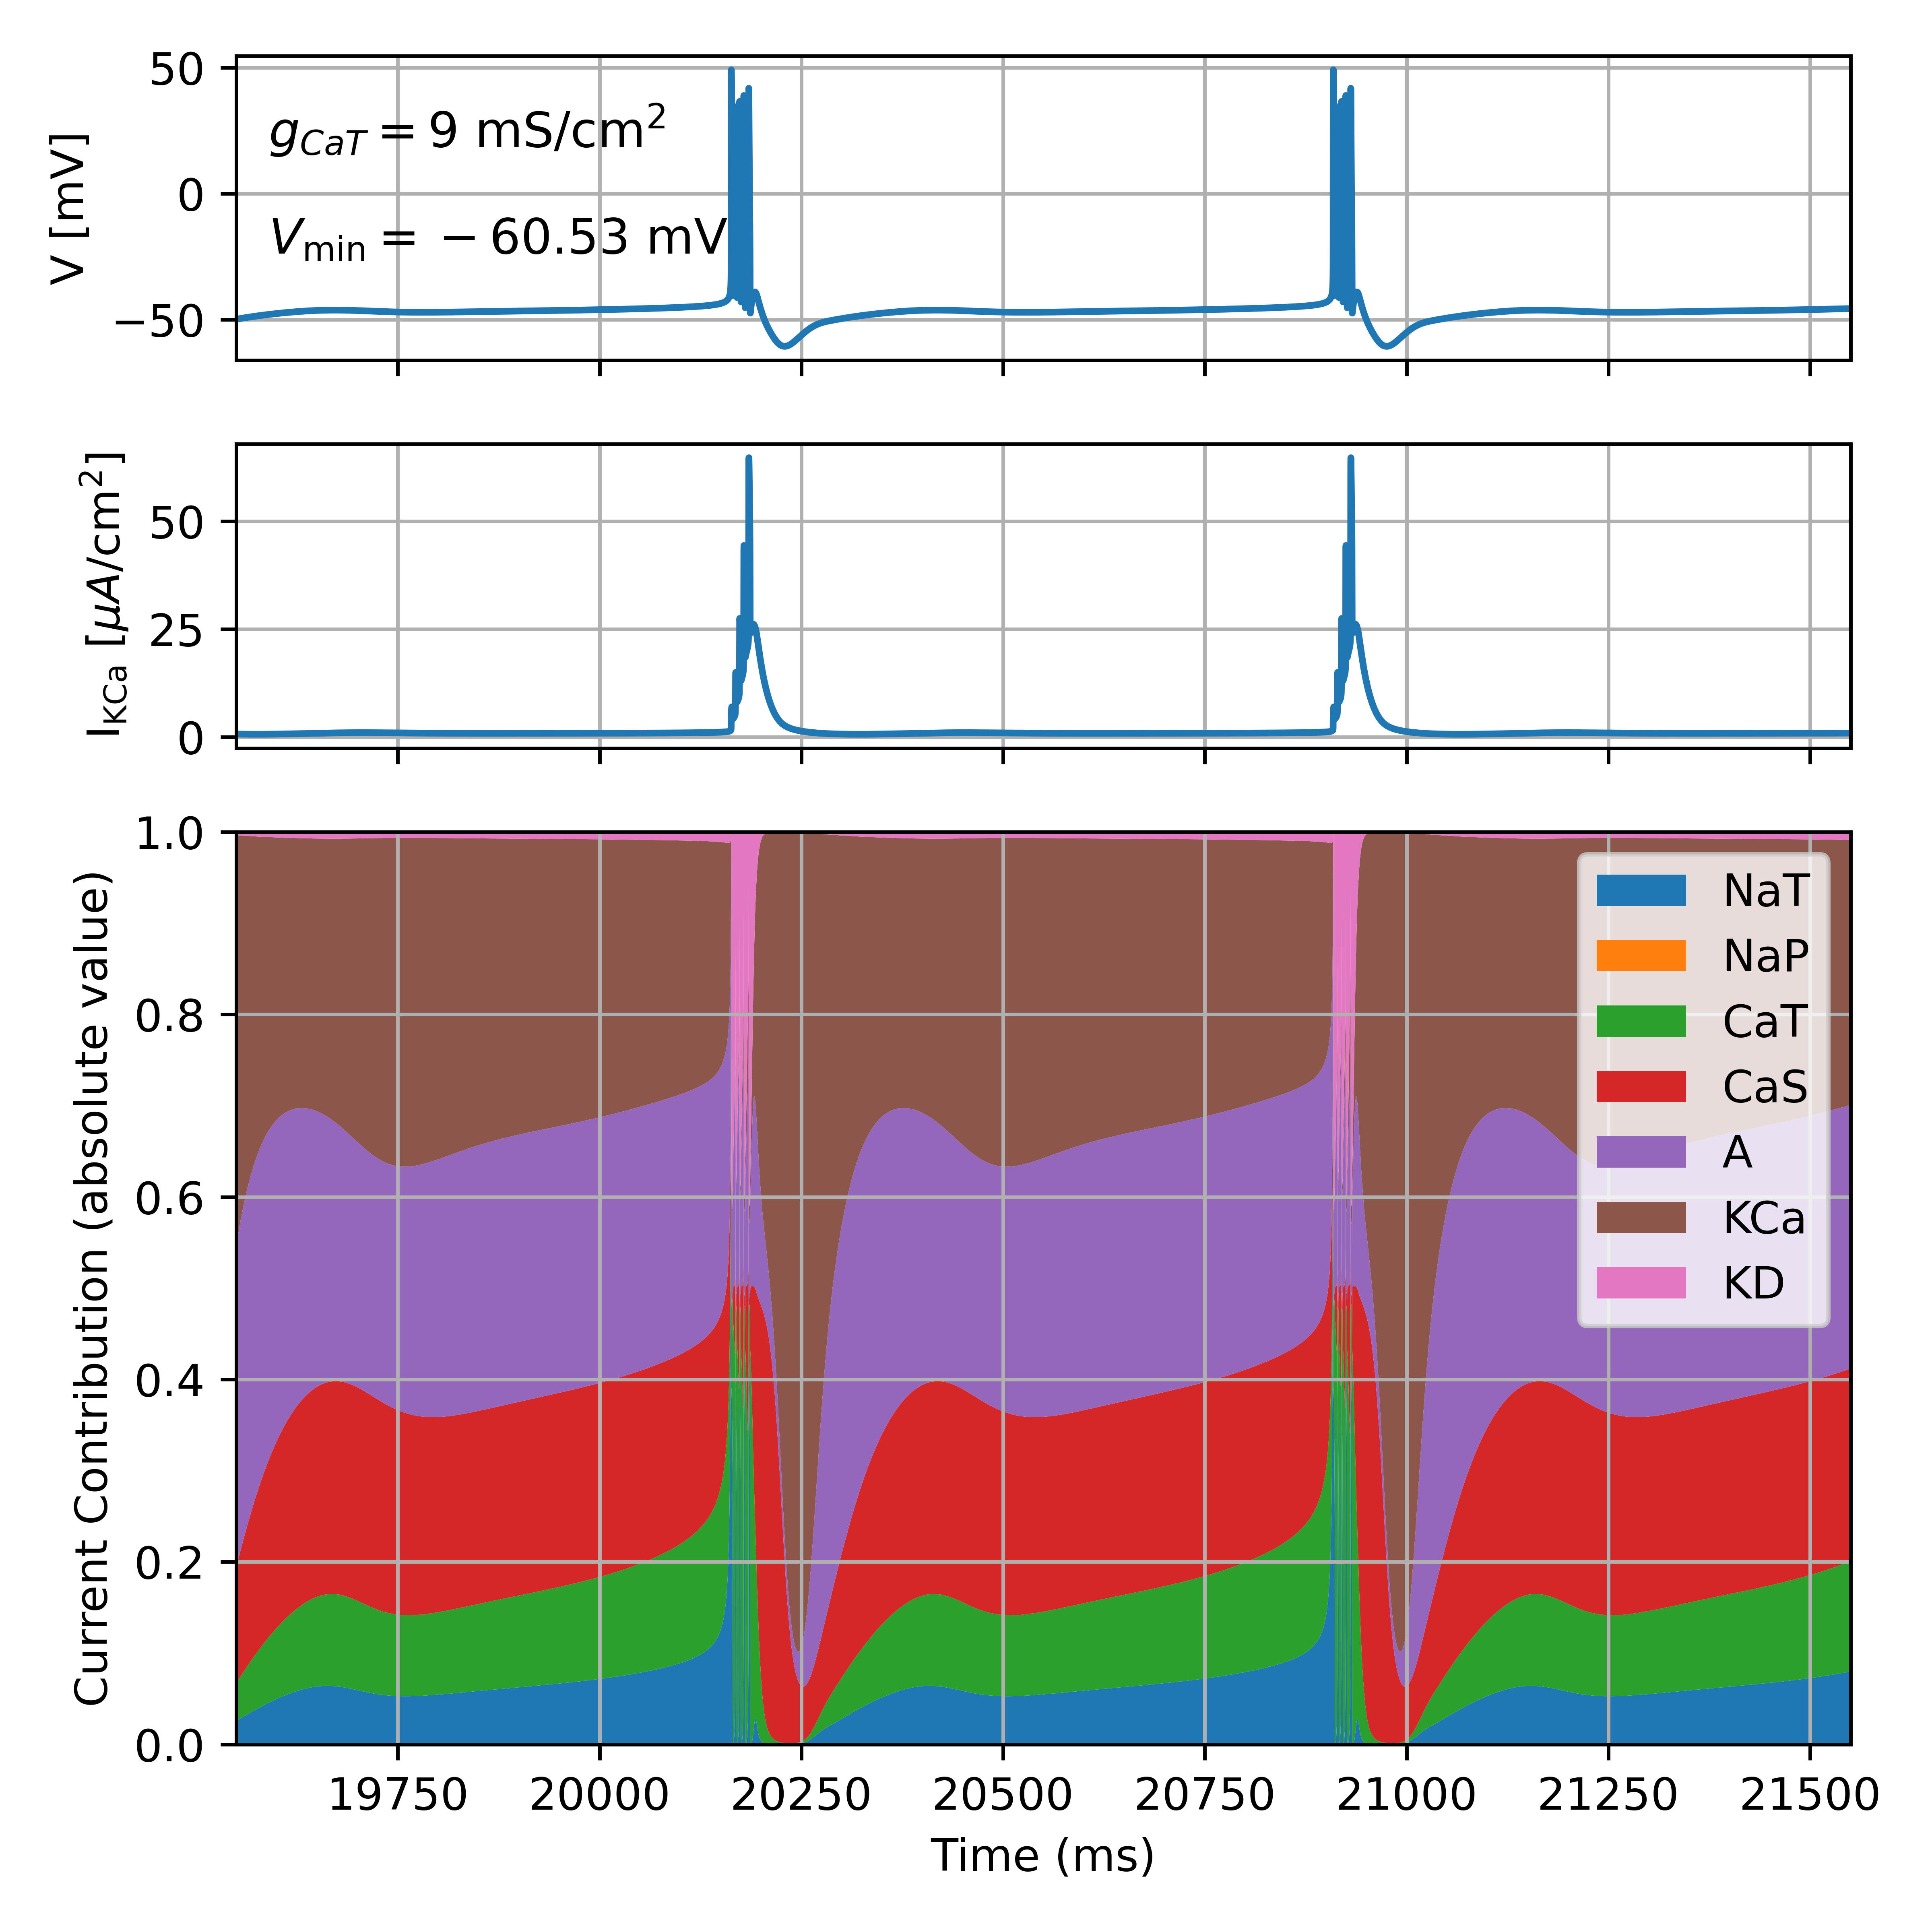
\includegraphics[width=\linewidth]{../img/rmp/goldman_1_g_9.png}
        \label{fig:rmp_models_contrib_10_goldman_1}
    \end{subfigure}
    \hfill
    \begin{subfigure}[t]{0.48\textwidth}
        \centering
        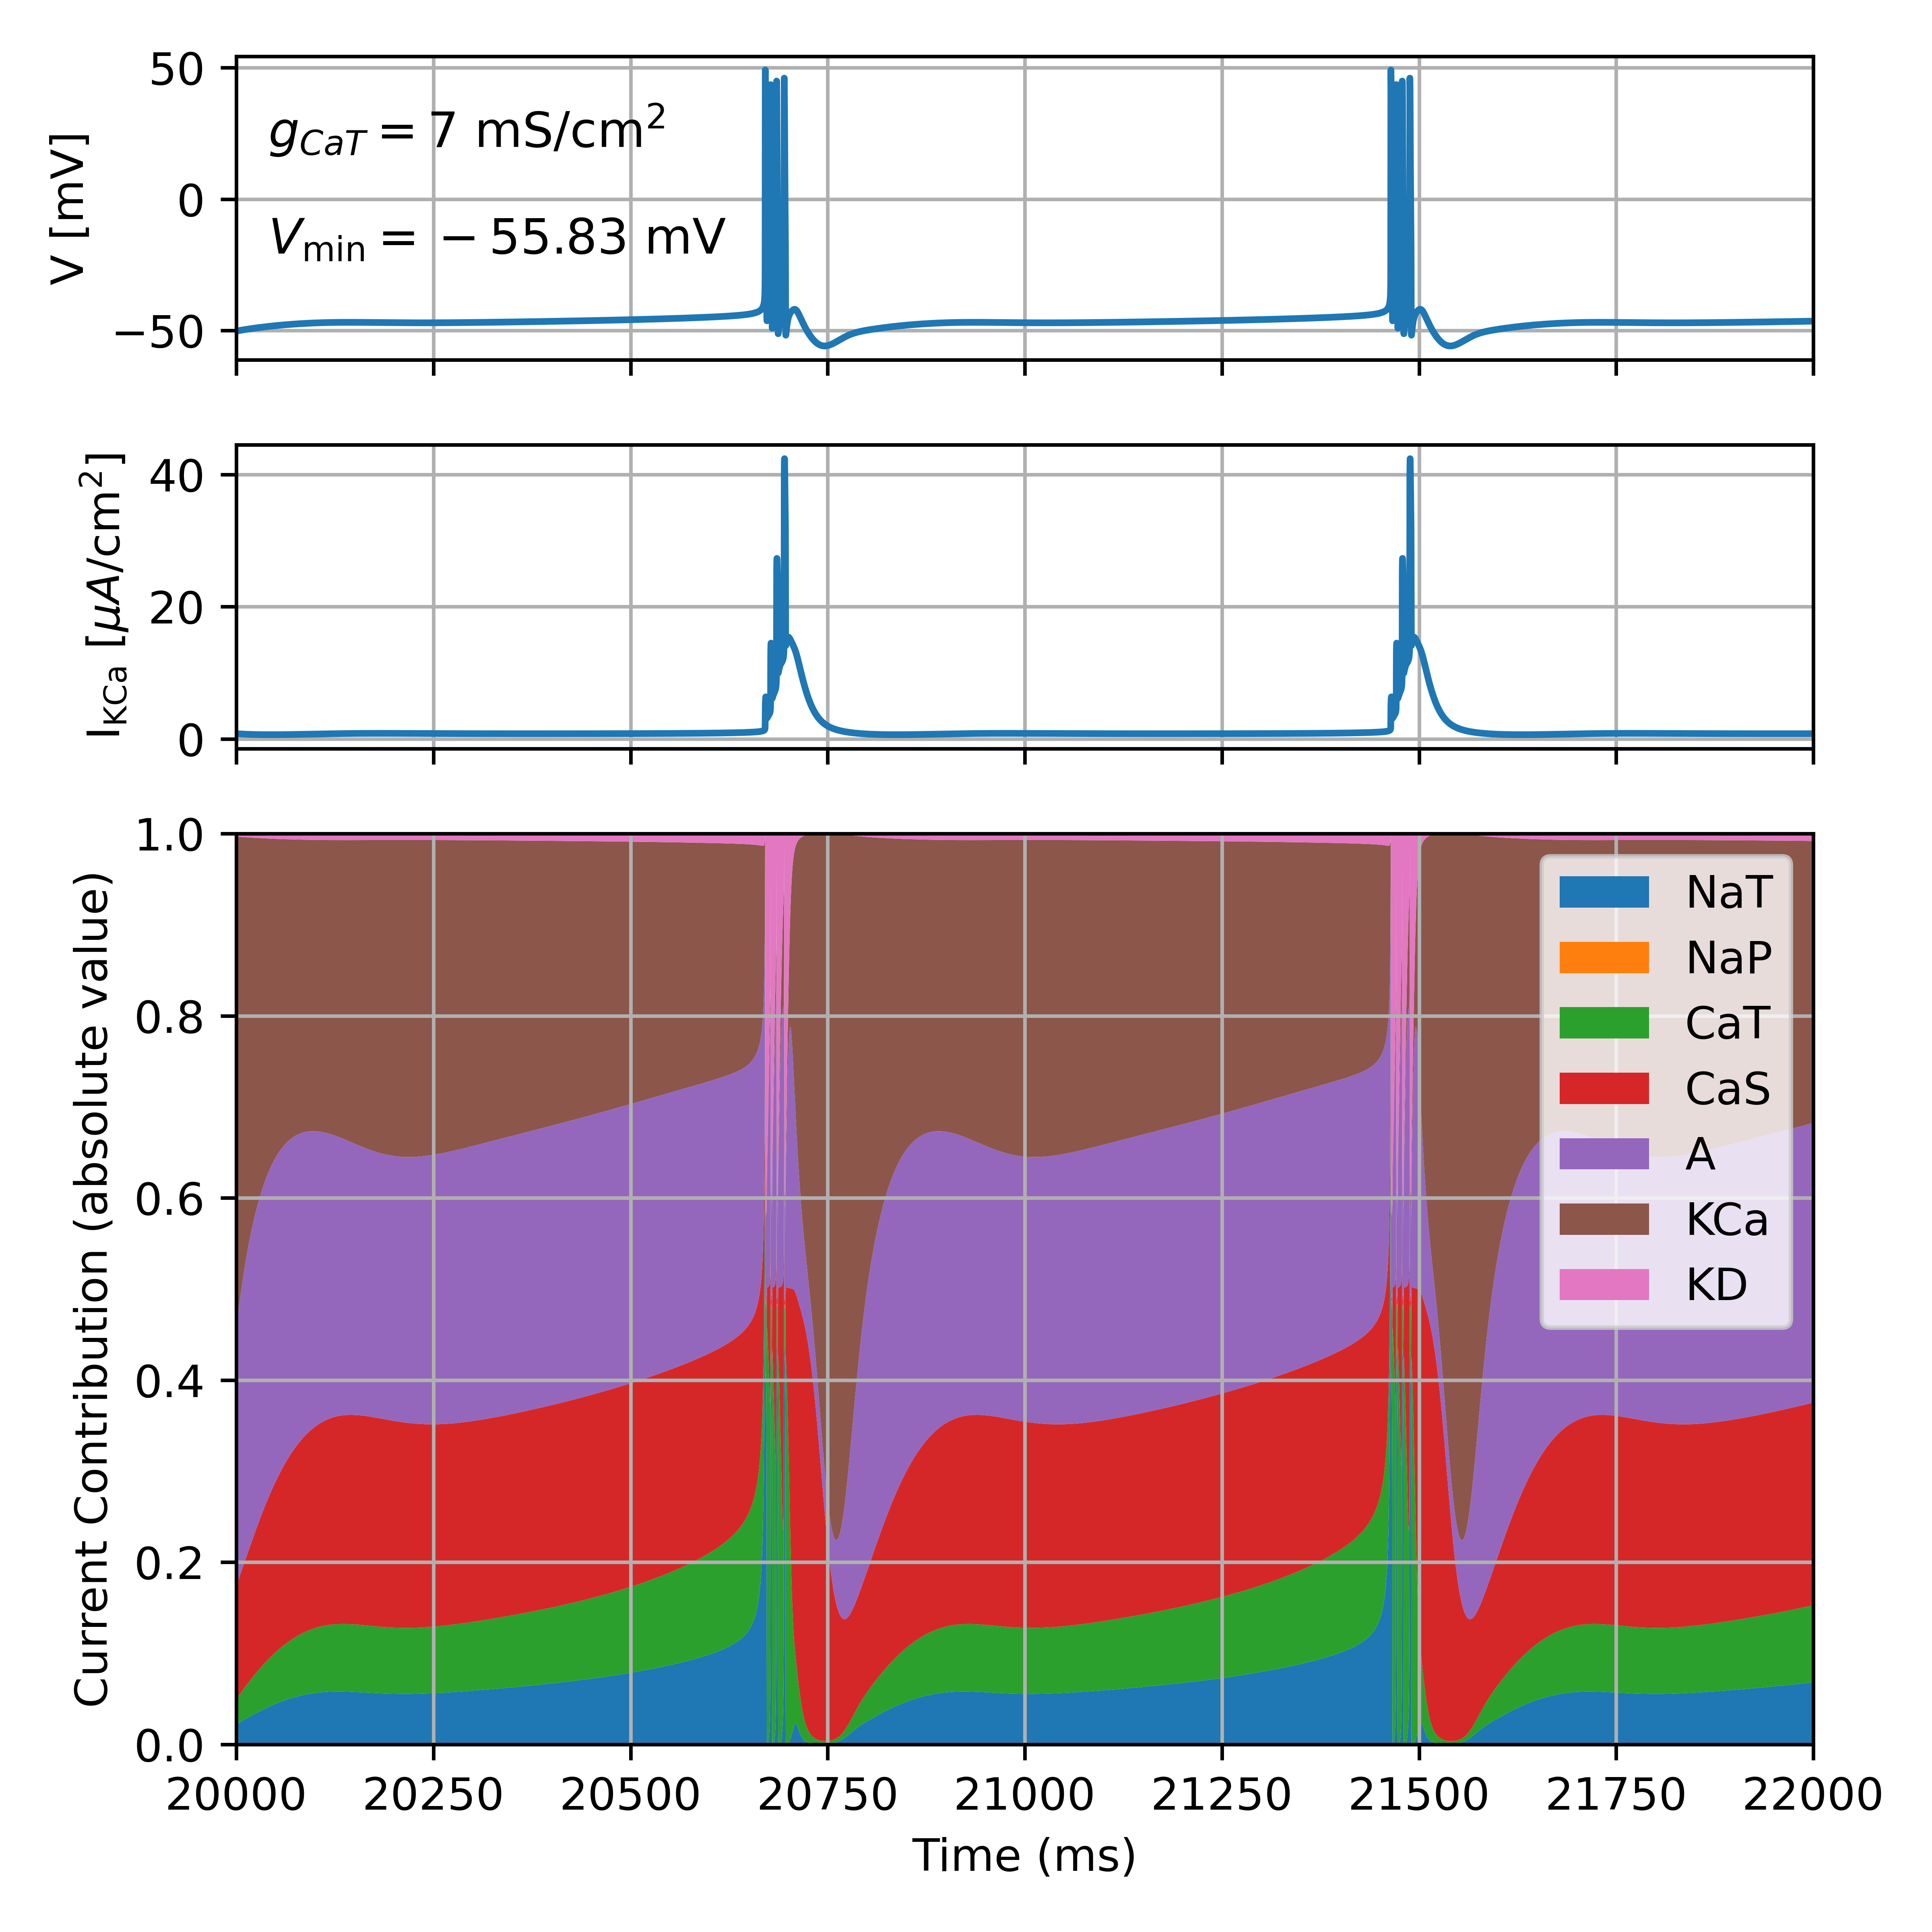
\includegraphics[width=\linewidth]{../img/rmp/goldman_1_g_7.png}
        \label{fig:rmp_models_contrib_5_goldman_1}
    \end{subfigure}

    \textbf{Goldman 2 Model} \\[1ex]  % Title at top center

    % First row
    \begin{subfigure}[t]{0.48\textwidth}
        \centering
        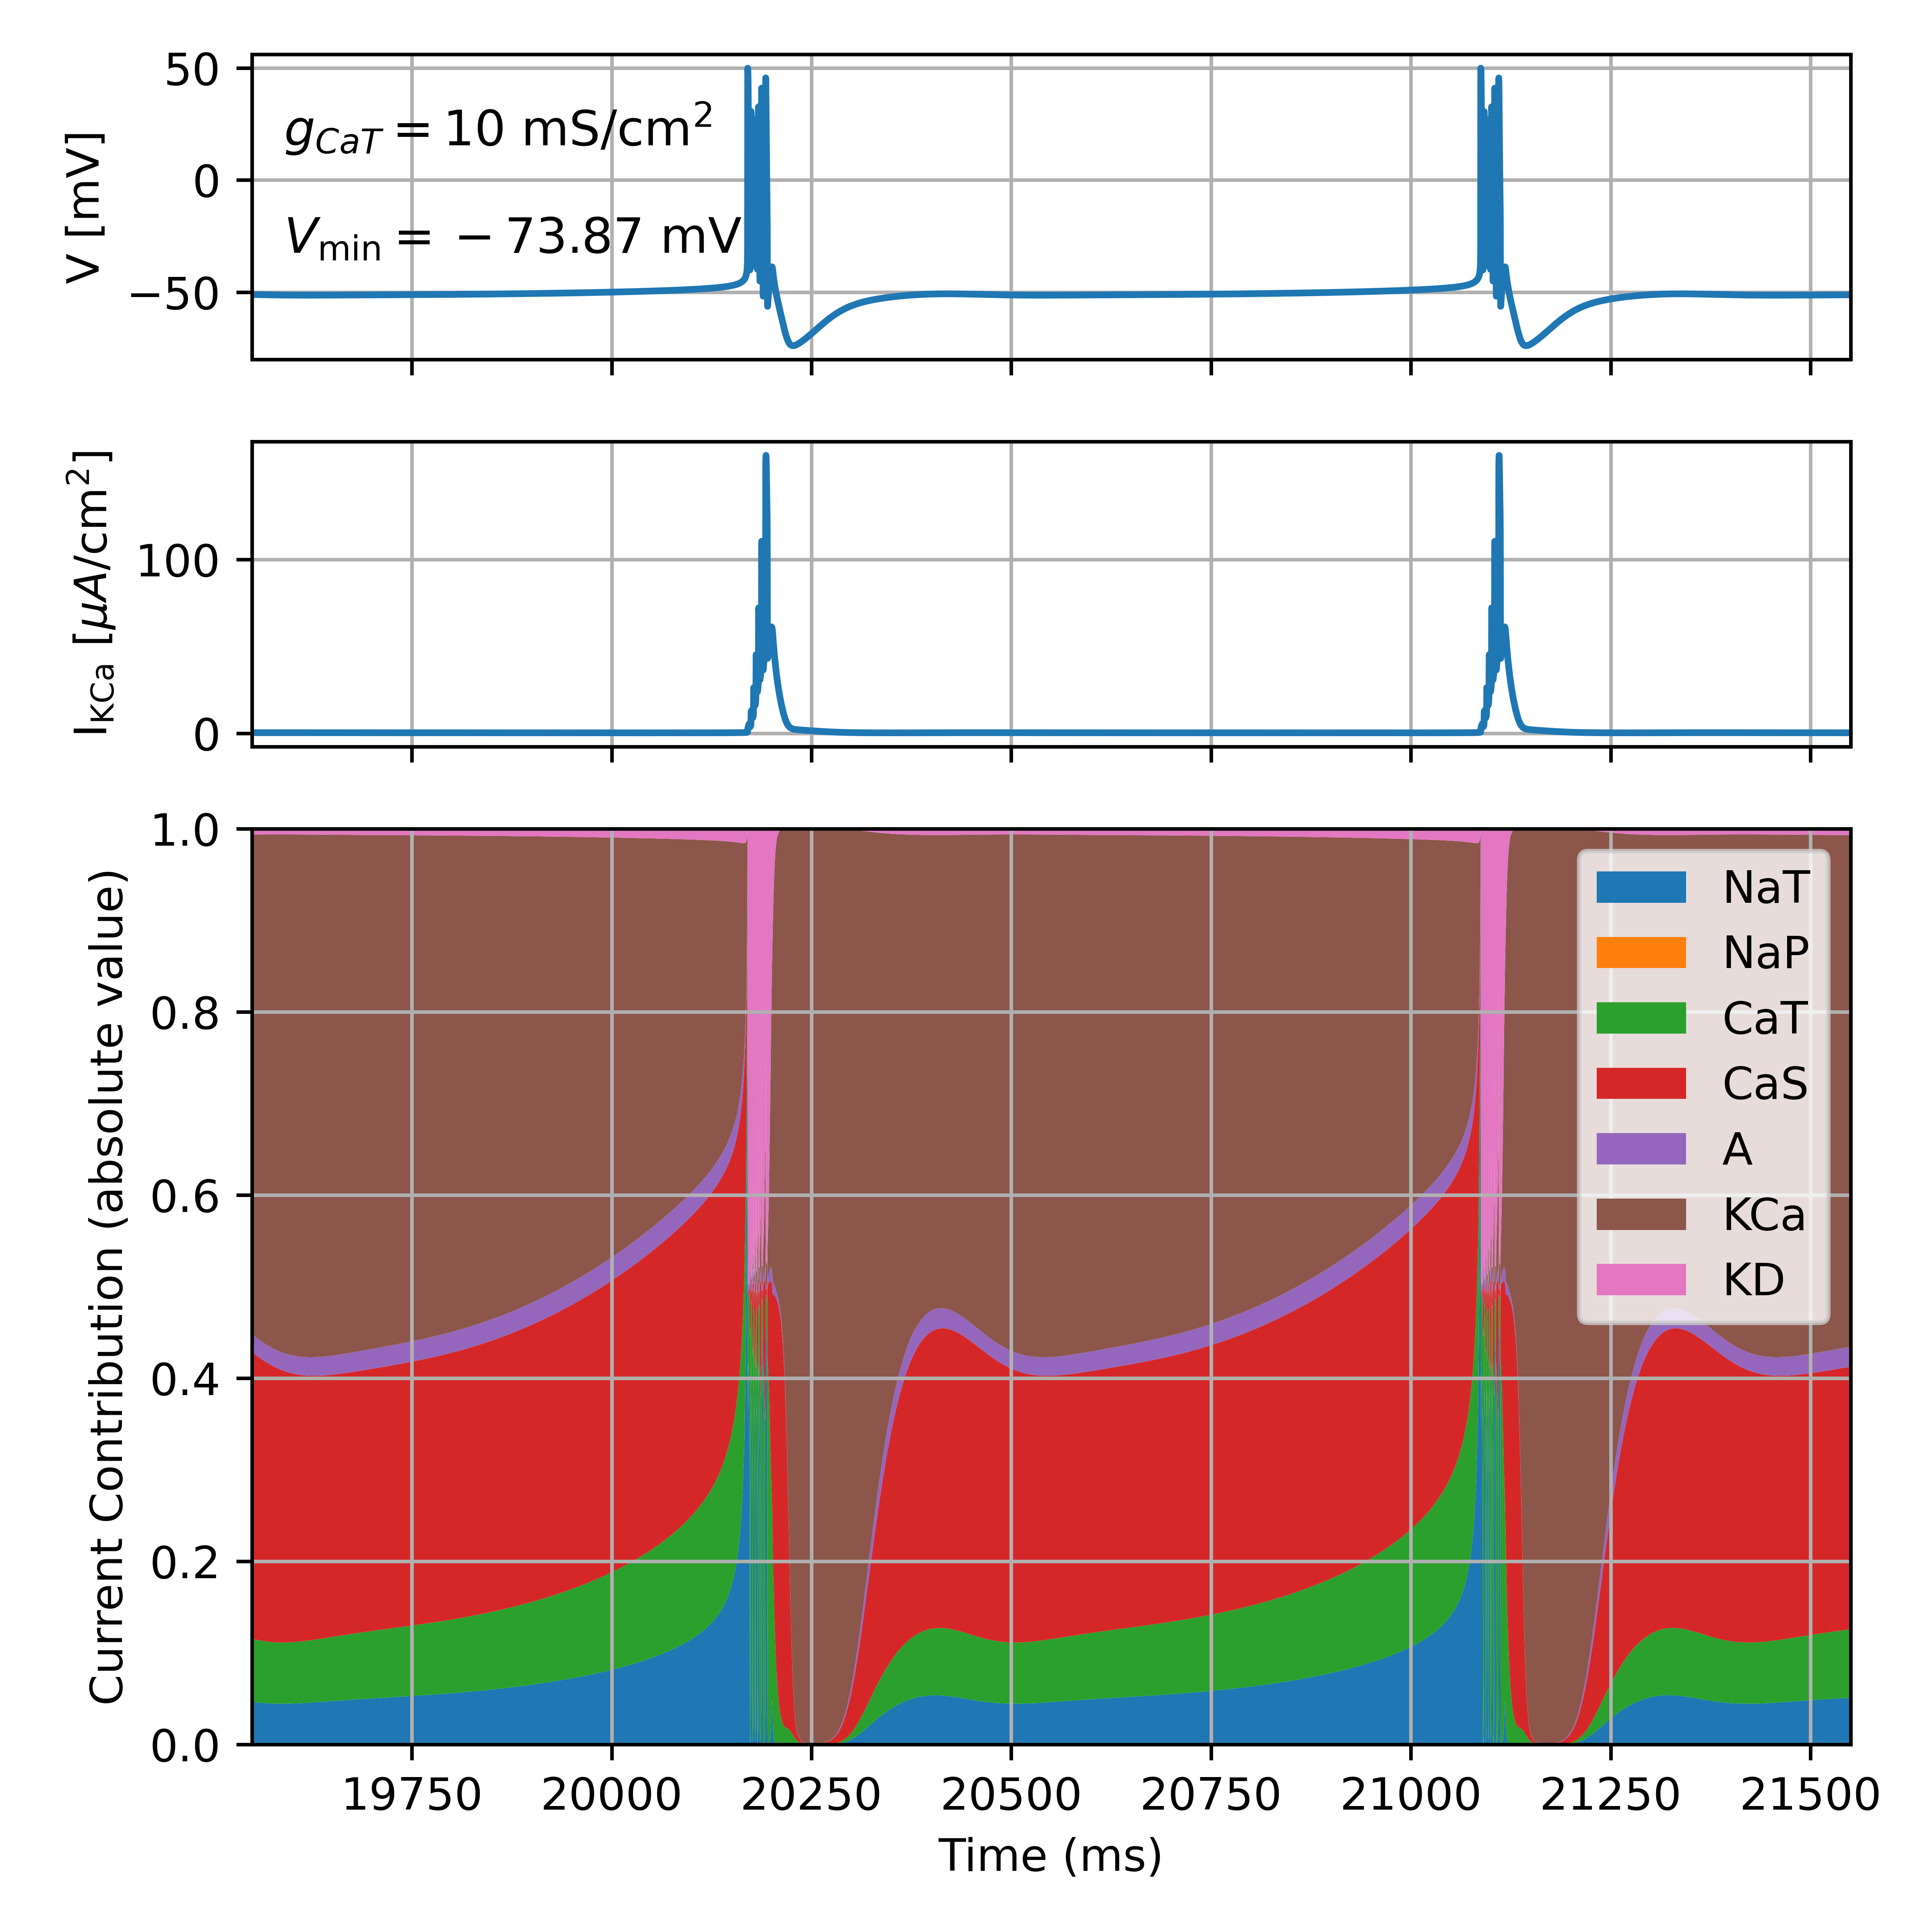
\includegraphics[width=\linewidth]{../img/rmp/goldman_2_g_10.png}
        \label{fig:rmp_models_contrib_10_goldman_2}
    \end{subfigure}
    \hfill
    \begin{subfigure}[t]{0.48\textwidth}
        \centering
        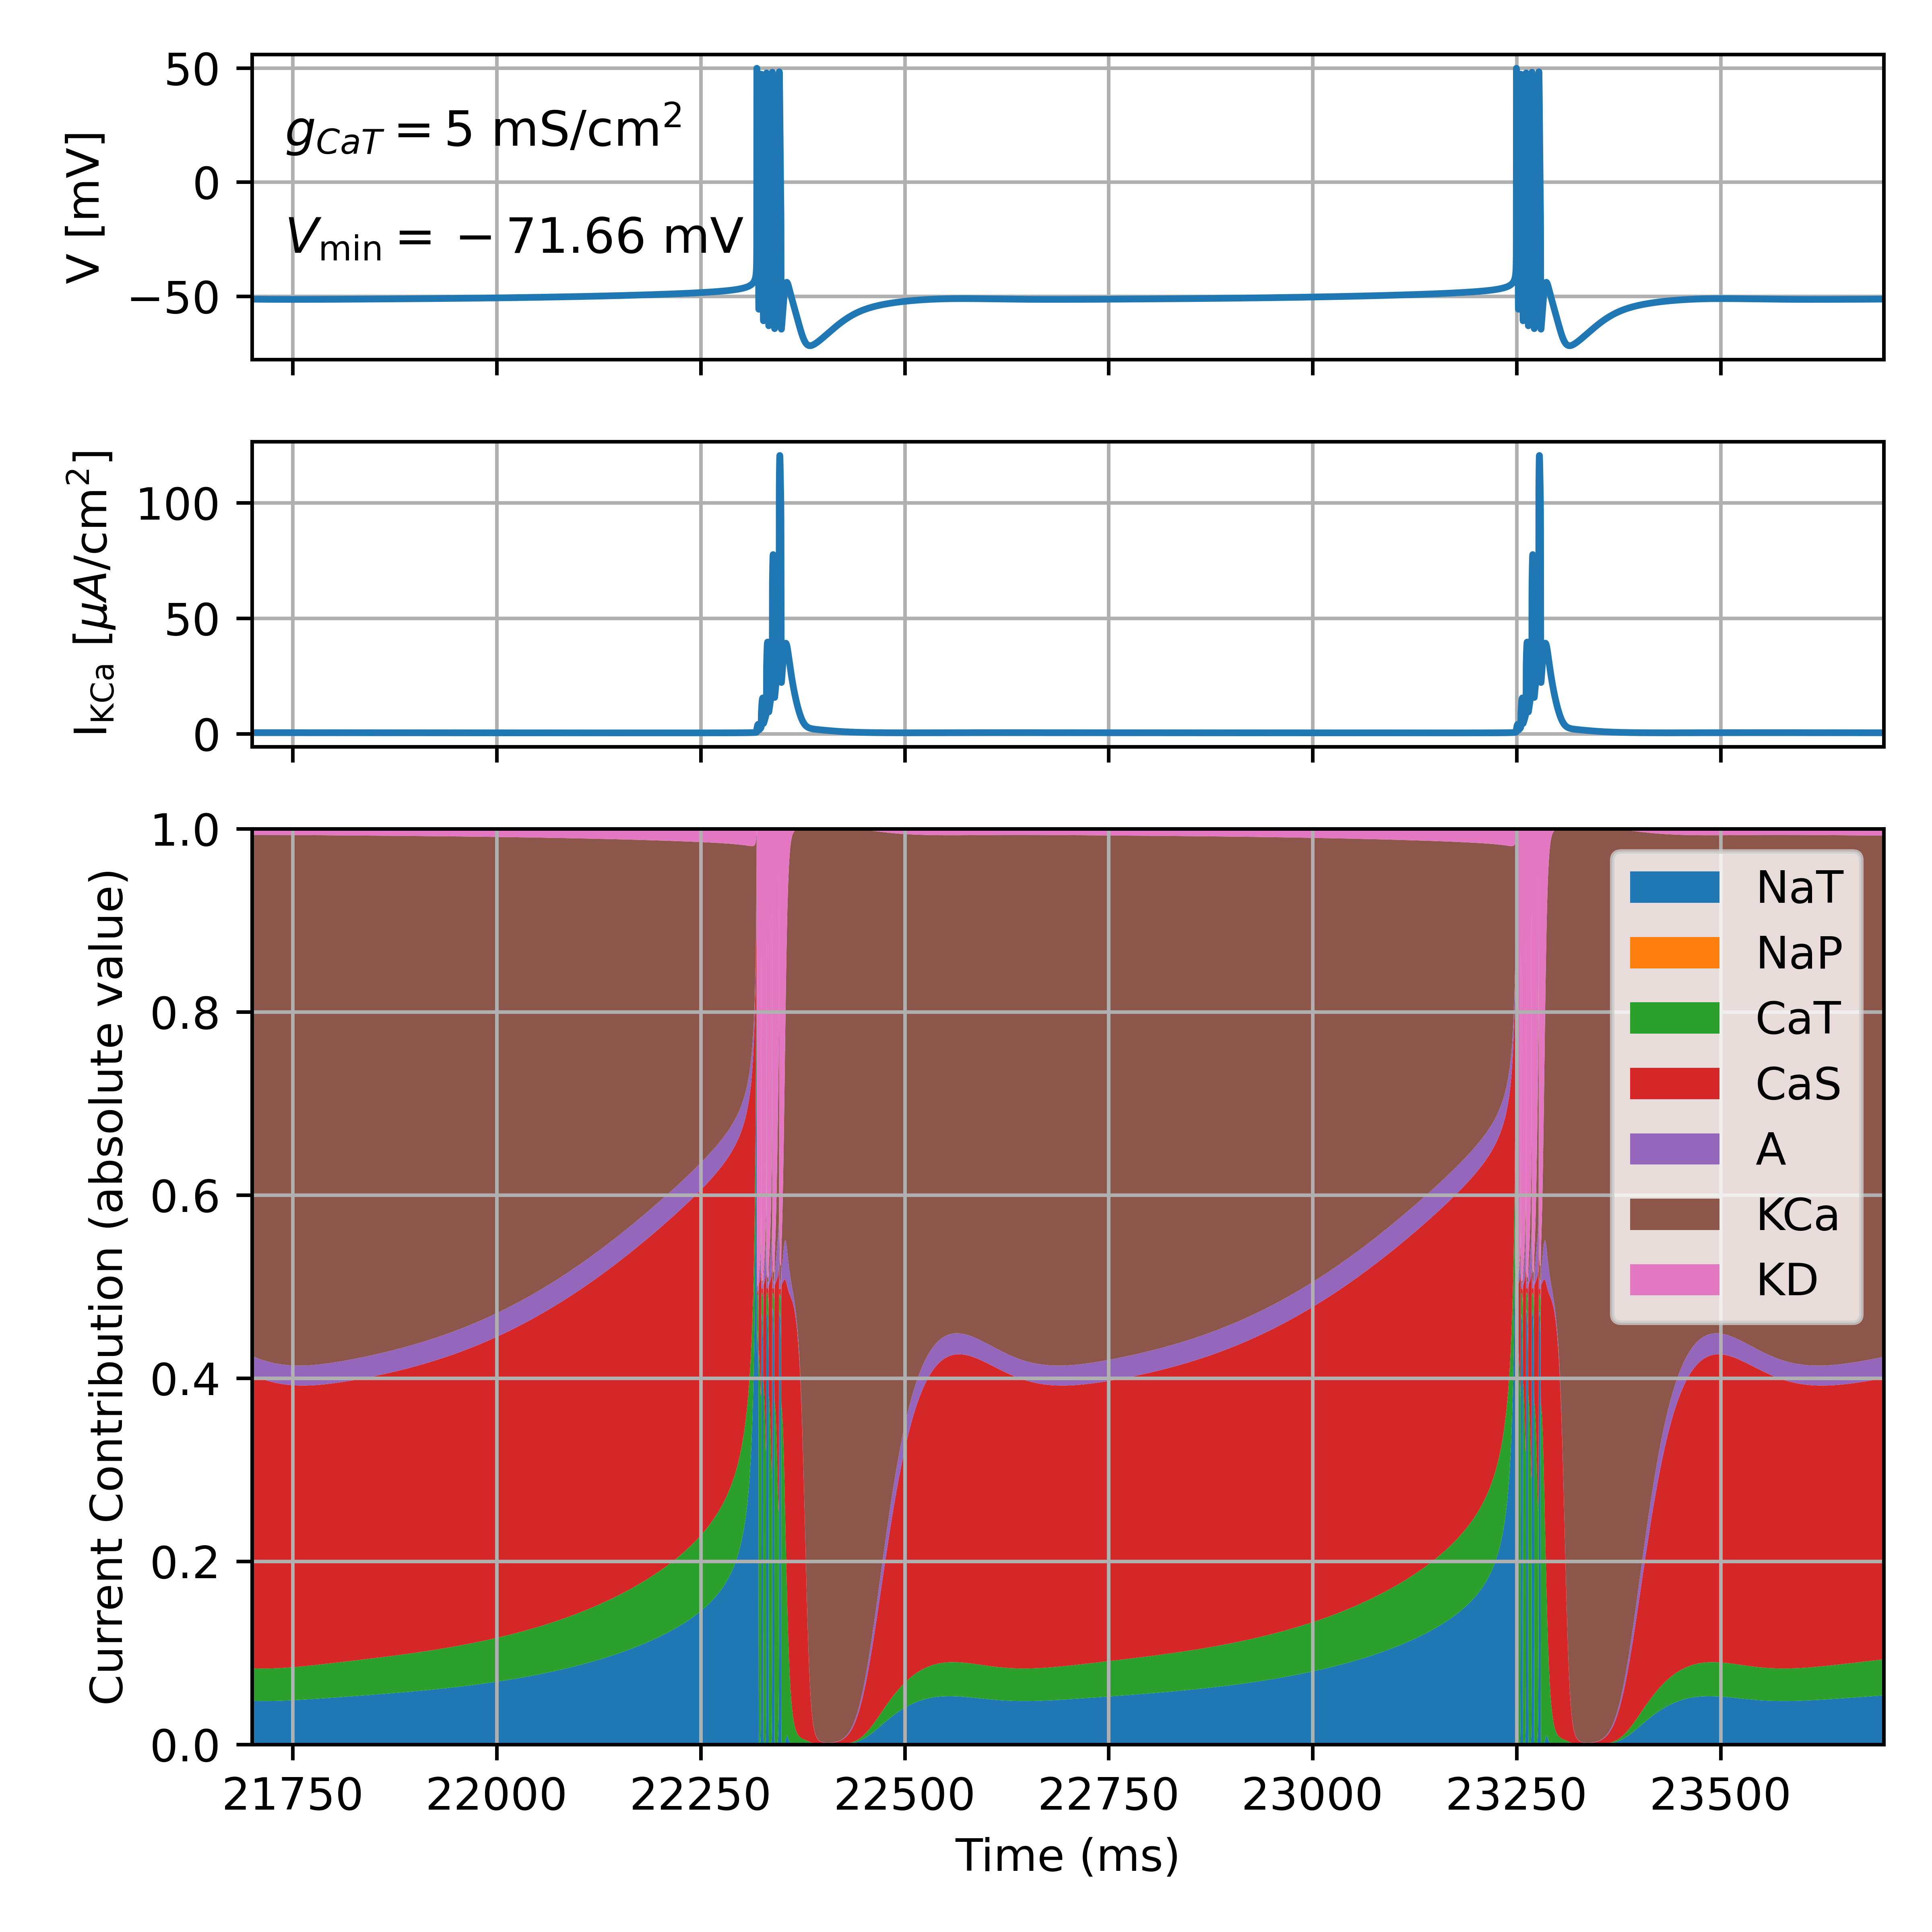
\includegraphics[width=\linewidth]{../img/rmp/goldman_2_g_5.png}
        \label{fig:rmp_models_contrib_5_goldman_2}
    \end{subfigure}
    
    \caption[Contribution of calcium-activated potassium channel on minimal membrane potential]{\textbf{Contribution of calcium-activated potassium channel on minimal membrane potential.} Results shown for the Goldman 1 and Goldman 2 models, with the external input current set to $1$ $\mu S/\text{cm}^2$ for Goldman 1, and to $0$ for the Goldman 2 model. Parameter values for the maximal conductance of the T-type channels are indicated as text in each figure. All other parameters were held constant, as described in Appendix \ref{appendix:functions_and_parameters}. Top: voltage trace, with the corresponding minimal membrane potential indicated as text. Middle: current through the calcium-activated potassium channel (KCa). Bottom: stack plot showing the relative contribution of each ionic current at each simulation time step (see main text for details). \textcolor{red}{Adjust ylim}}
    \label{fig:rmp_models_contrib_fig_goldman}
\end{figure}
}



Figure \ref{fig:rmp_models_phase} illustrates the regions in the I$_{\text{ext}}-g_{CaT}$ parameter plane where each of the investigated models exhibited bursting behaviour. For these regions, the figure also shows the corresponding bursting period and the minimal membrane potential obtained from numerical simulations.

Several observations can be made from the figure. First, the modulation of the minimal membrane potential by the maximal conductance of the T-type calcium channels is more pronounced in the Goldman 1 model in comparison to the Goldman 2 model. Second, there are regions where the minimal membrane potential changes abruptly with variations in T-type conductance. Third, when decreasing the maximal conductance of the T-type channel, the minimal membrane potential drops, rather than increases, near the transition from bursting to spiking (comare the regions outlined by the red curve to the area in the left plot where the model transitions from bursting (red) to spiking (blue); this effect is illustrated more clearly in Figure \ref{fig:rmp_models_phase_i_slices}). These aspects will be further discussed in the remainder of this section.


\subsubsection{Contribution by calcium-activated potassium channel}

\noindent To investigate whether calcium-activated potassium channels are responsible for the increase in the minimal membrane potential observed in Figure \ref{fig:rmp_models_phase}a-b, the relative contribution of each current was analyzed in representative simulations in which the model exhibited approximately $1$ Hz bursting.

The contribution of each current was defined as the percentage of its magnitude relative to the sum of the absolute values of all ionic currents. The results are shown in Figure \ref{fig:rmp_models_contrib_fig} for the Goldman 1 and Goldman 2 models, along with the corresponding voltage trace and the current through the calcium-activated potassium channel (KCa). In the stack plots, the height of each colored region represents the percentage of the magnitude of that current relative to the total ionic current at each time point of the simulation.


As shown in Figure \ref{fig:rmp_models_contrib_fig_goldman}, in all cases the minimal membrane potential is primarily affected by the calcium-activated potassium channel, which contributes the largest fraction of the total current at that time (Goldman 1: $77.53\%$ for $g_{CaT}=7$ mS/cm$^2$ and $89.82\%$ for $g_{CaT}=9$ mS/cm$^2$; Goldman 2: $99.92\%$ for $g_{CaT}=10$ mS/cm$^2$ and $99.82\%$ for $g_{CaT}=5$ mS/cm$^2$).

Interestingly, although the minimal membrane potential was more strongly mediated by calcium-activated potassium channels in the Goldman 2 model, Figure \ref{fig:rmp_models_phase} shows that the modulation of the minimal membrane potential is more pronounced in the Goldman 1 model. Furthermore, as illustrated in Figure \ref{fig:rmp_models_contrib_fig_goldman}, the contribution of the KCa channel is more robust to changes in T-type conductance in the Goldman 2 model. Specifically, reducing the conductance from $10$ mS/cm$^2$ to $5$ mS/cm$^2$ in the Goldman 2 model has a smaller effect on the KCa contribution than reducing it from $9$ mS/cm$^2$ to $7$ mS/cm$^2$ in the Goldman 1 model.

The Goldman 1 and Goldman 2 models differ only by the maximal conductances of the ion channels (see Appendix \ref{appendix:functions_and_parameters}, and Figure \ref{fig:model_conductances}). Apart from differences in other conductances, the maximal conductance of calcium activated potassium channels are lower in Goldman 1 in comparison to Goldman 2 models (Goldman 1: $g_{CaT}=7$, $g_{KCa}=25$; Goldman 2: $g_{CaT}=10$, $g_{KCa}=40$). Even a small influx of calcium could potentially result in domination of the KCa-mediated currents if the maximal conductance of the KCa channels is large enough.

\color{red}

To test this - vary g\_CaT + g\_KCa and: (Todo) 1. (!IMPORTANT!) Plot similar figures as in Figure \ref{fig:rmp_models_phase}, but with colour showing total calcium influx during burst, total t-type current during burst, total t-type current during burst, total calcium current during burst, total KCa current after burst before plateau.
BUT: x axis - CaT channel and y axis KCa to see how the calcium AND KCa conductance affects resting membrane potential

\color{black}


\subsubsection{Abrupt shifts and non-monotonic trends in minimal membrane potential}

\noindent Figure \ref{fig:rmp_models_phase} illustrates that in certain regions of the I$_{\text{ext}}-g_{CaT}$ parameter space, decreasing the maximal conductance of the T-type channels leads to a decrease in the minimal membrane potetial contrary to the behaviour observed for larger values of $g_{CaT}$. This effect is more clearly visible in Figure \ref{fig:rmp_models_phase_i_slices}, where the minimal membrane potential is plotted against the maximal conductance of the T-type channel at fixed external input current.

To better understand this behaviour, representative voltage traces were examined around the critical point where the minimal membrane potential begins to decrease as $g_{CaT}$ is reduced (Figure \ref{fig:rmp_models_phase_i_slices_voltage}). The figure shows that this drop in minimal potential corresponds to the presence of spike undershoots that fall below the membrane potential at rest (i.e. potential where the model neurons do not exhibit spikes).

Since in R5 neurons the membrane potential during bursts is strictly greater than during the interburst interval, could the above-described result indicate a partial blockade of the T-type channels?
Not necessarily. As illustrated in Sections \ref{sec:sleep_and_r5_network} and \ref{sec:math_background}, even within the low-dimensional fast-slow system framework, bursting can arise through various mechanisms, depending on the nature of burst onset and offset. Moreover, variation in the maximal conductances of single channels has been shown to produce qualitatively different effects, even within the same model, when operating in different parameter regimes - despite exhibiting similar voltage traces under default parameters (i.e. before the variation in single conductances) \parencite{alonsoVisualizationCurrentsNeural2019}. Thus, this effect is likely model-specific rather than general. Since this region does not appear to be relevant in understanding the electrophysiological properties of the R5 neurons, it was not analyzed further.


\begin{figure}[!t]
    \centering
    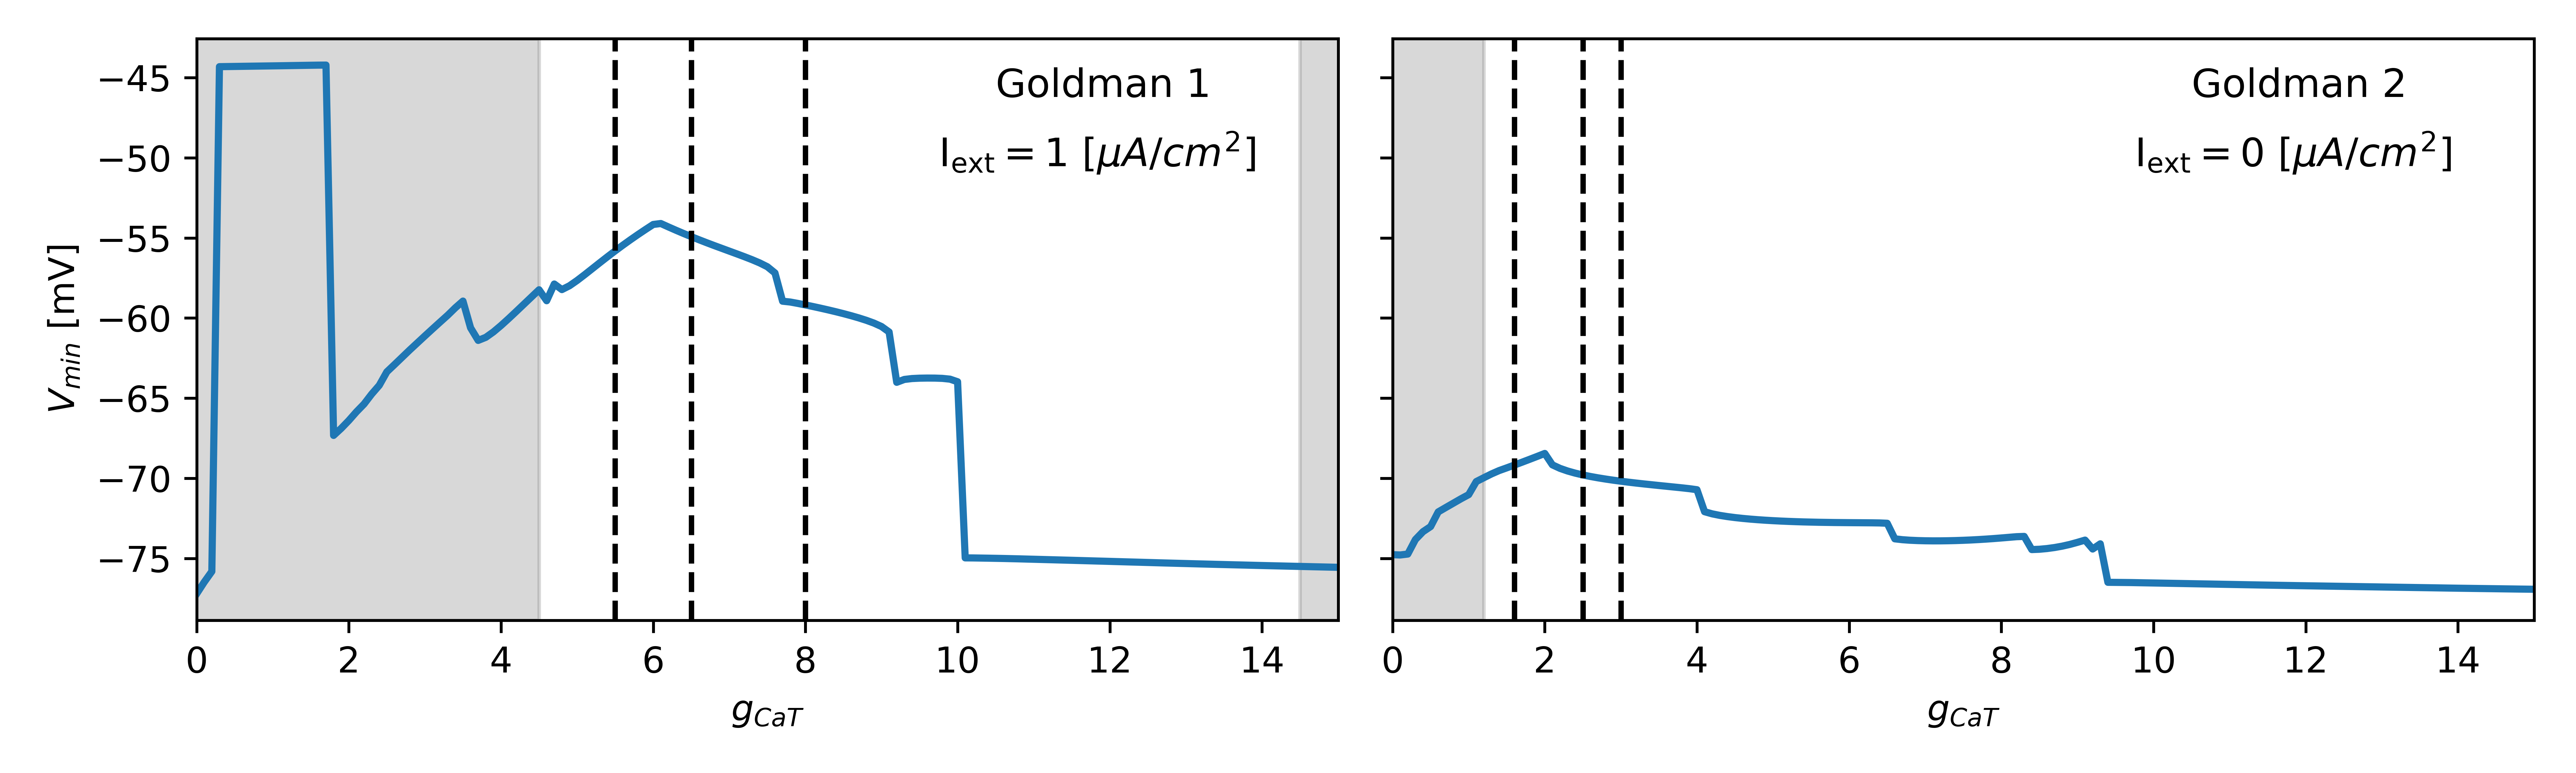
\includegraphics[width=0.9\linewidth]{../img/rmp/goldman_1_2_i_slices.png}
    \caption[Dependence of minimal membrane potential on T-type conductance]{\textbf{Dependence of minimal membrane potential on T-type conductance.} The figure shows the values of the minimal membrane potential along a horizontal slice of the corresponding heatmap shown in Figure \ref{fig:rmp_models_phase}ab for the Goldman 1 (left) and Goldman 2 (right) models. The corresponding values of the external current are indicated by the text within each plot. Grey areas represent regions where the models did not exhibit bursting behaviour. Vertical dashed lines indicate the parameter values for the T-type conductance for which the simulated membrane potential traces are shown in Figure \ref{fig:rmp_models_phase_i_slices_voltage}.}
    \label{fig:rmp_models_phase_i_slices}
\end{figure}

\begin{figure}[!t]
    \centering
    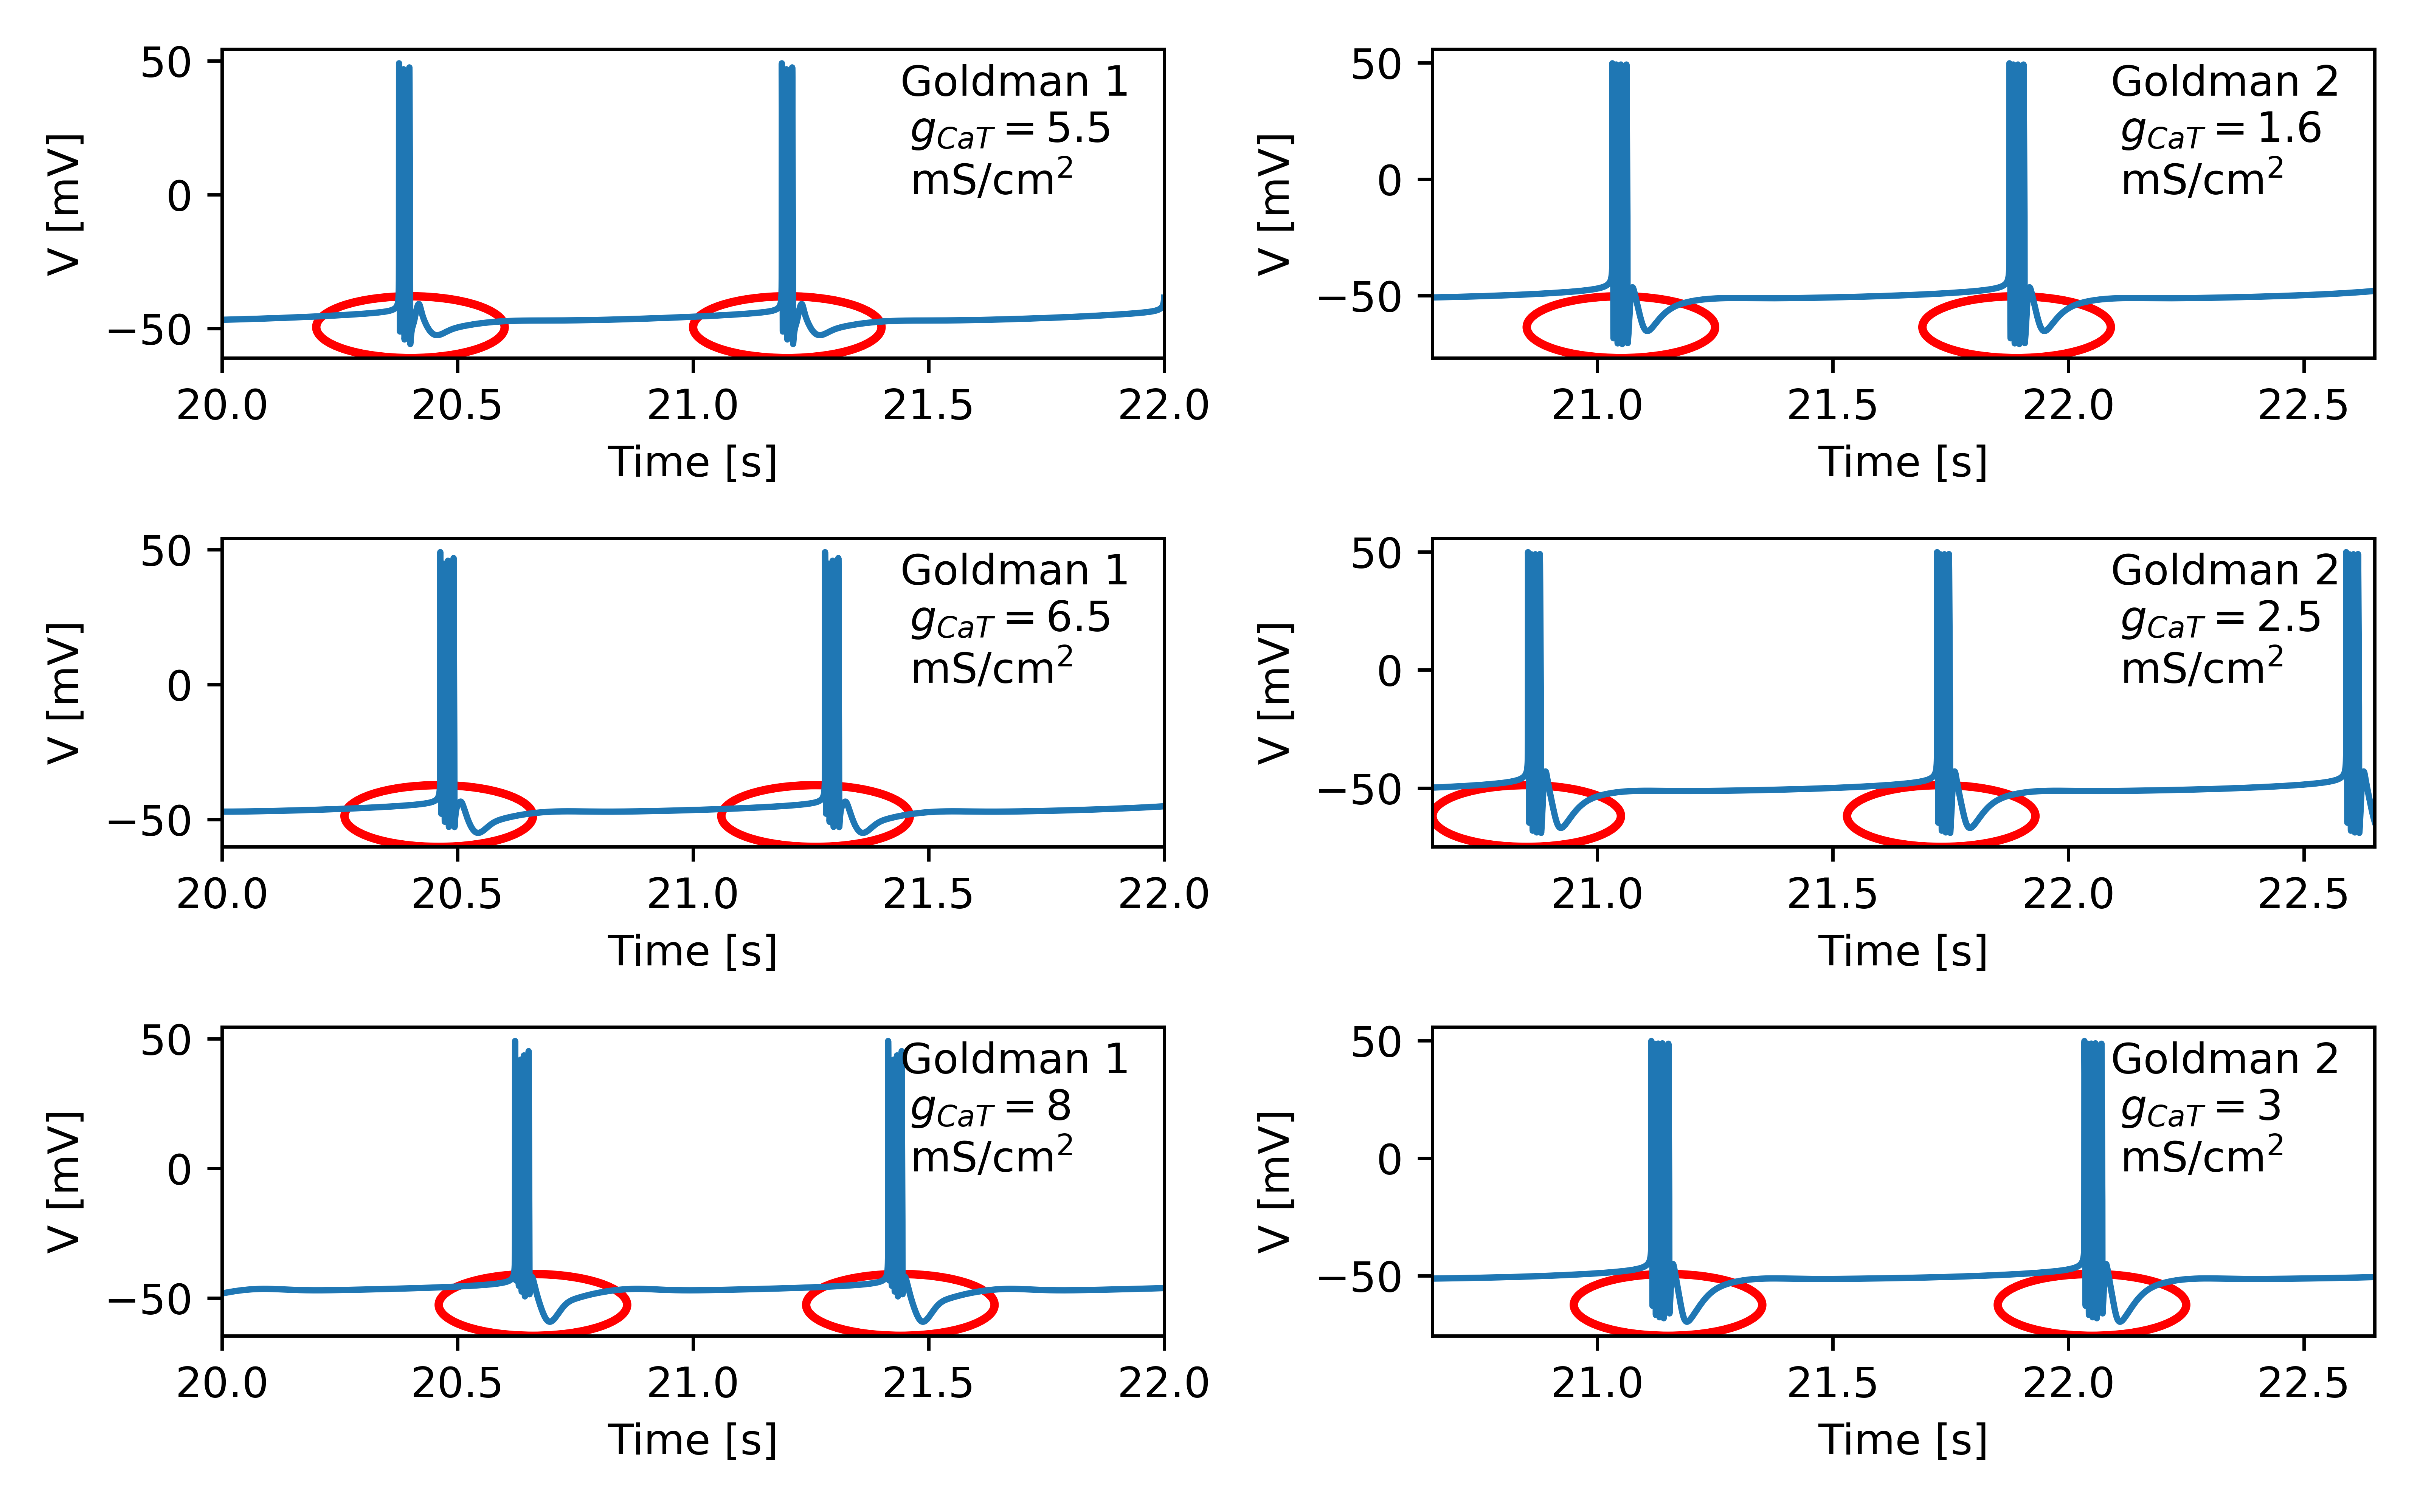
\includegraphics[width=0.9\linewidth]{../img/rmp/goldman_1_2_i_slices_vtraces.png}
    \caption[Voltage traces across the turning point in minimal membrane potential]{\textbf{Voltage traces across the turning point in minimal membrane potential.} The figure shows representative voltage traces of the model neurons for parameter values corresponding to the dashed lines in Figure \ref{fig:rmp_models_phase_i_slices}. For both models, the region where the minimal membrane potential decreases with decreasing maximal conductance of the T-type calcium channels corresponds to the case where the spikes exhibit undershoot below the membrane potential at rest (i.e. when the model neuron exhibits no spikes).}
    \label{fig:rmp_models_phase_i_slices_voltage}
\end{figure}

\color{red}



2. If have time after finishing everything else: add "non-biologically plausible" calcium current to wang: steap activation time constant as for EAG, but with longer time constant to see the effect there. The result will not change much, maybe one more sentence in the discussion.

\color{black}

\newpage
\begin{figure}[H]
    \centering
    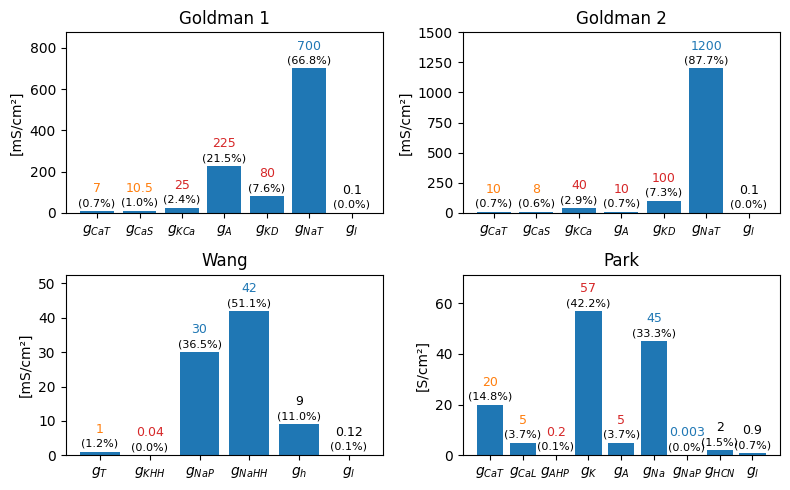
\includegraphics[width=\linewidth]{../img/materials_and_methods/model_conductances.png}
    \caption[Default maximal conductances of the models described]{
        \textbf{Default maximal conductances of the models described.} Labels on the $x$ axis correspond to ion channel names as described in the respective models (see Appendix \ref{appendix:functions_and_parameters} for a detailed description of the models).
        The numbers above each bar indicate the corresponding maximal conductance values, while the percentages below represent their relative value compared to all other channels in the same model.
        Colours indicate the ion permeability of each channel: orange for calcium, red for potassium, blue for sodium, and black for other currents (h-current and leak).
        Among all channels, the T-type calcium channels (labelled as $CaT$ in Goldman and Park models, and $T$ in the Wang model), and calcium-activated potassium channel (labelled as $KCa$ in the Goldman models and $AHP$ in the Park model) are of particular interest in the context of this work. Note that the original Wang model does not include a calcium-activated potassium channel. \textcolor{red}{This image will be in materials and methods, adding here for a reference}
    }
    \label{fig:model_conductances}
\end{figure}
    

\end{document}